\documentclass[usenames,dvipsnames,letterpaper,landscape,final]{slides}

\def\fileHome{.}
\def\icons{\fileHome/icons}

\input mySlideStyle2019-1.tex
\def\myfboxBlack#1{\fboxrule2pt\fbox{$\ds#1$}}
\newcommand\topSeparatorHeading[1]{\noPagetrue\begin{myslide}\headingline\vbox to5.5in{%
\vfil\begin{center}{{\large\myfboxBlack{\myfboxBlack{%
\text{\ \ \bf\Blue{\begin{tabular}{c}#1\end{tabular}\ \ }}}}}}%
\end{center}\vfil}\end{myslide}\noPagefalse}

\usepackage{multirow}
\usepackage{enumitem}
\usepackage[ruled,vlined]{algorithm2e}
%\usepackage{wallpaper}
		  \usepackage{mathtools}

\newcounter{outlineNumber}\setcounter{outlineNumber}{0}
\def\outno{\stepcounter{outlineNumber}\Blue{\theoutlineNumber. }}

\definecolor{boxColor}{rgb}{.4, .05, .2}

%------------------------------------------------------------------------------
\tikzset{cross/.style={cross out, draw=black, minimum size=2*(#1-\pgflinewidth), inner sep=0pt, outer sep=0pt},cross/.default={1pt}}

\renewcommand\floatpagefraction{0}
\renewcommand\textfraction{0}
\renewcommand\topfraction{1}
\renewcommand\bottomfraction{1}
\setcounter{topnumber}{10}
\setcounter{bottomnumber}{10}
\setcounter{totalnumber}{10}

\def\picWidth#1#2{\includegraphics[clip=true,keepaspectratio=true,width=#1]{#2}}
\def\picHeight#1#2{\includegraphics[clip=true,keepaspectratio=true,height=#1]{#2}}
\def\picWidthHeight#1#2#3{\includegraphics[clip=true,width=#1,height=#2]{#3}}

%\let\itemOld=\item
%\def\item{\parskip=0pt\itemsep=0pt\itemOld}
\begin{document}
\begin{myslide}
\headingline
		  %\vspace*{-30pt}
		  {\bf\Large\begin{center}
					 %Simulation of Partial Melting Mantle
Simulation of Flow and Transport in the Partially Molten Mantle of the Earth
		  \end{center}}

\vfill

\begin{center}{\small\obeylines
Chenyu Tian
\bigskip
%		  {\it\OliveGreen{CSEM} 
%		  \Blue{\it Oden Institute}}
%\BurntOrange{The University of Texas at Austin}}
		  {Oden Institute, University of Texas at Austin}}
\end{center}

\vfill

{\small\begin{center}
					 Todd Arbogast, Oden Institute \& Mathematics, University of Texas at Austin\\
Marc A. Hesse, Oden Institute \& Geosciences, University of Texas at Austin\\
		  \end{center}}

		  \vspace*{40pt}

\end{myslide}

% =============================================================================

\begin{myslide}
          \heading{Motivation}
          \parbox{0.6\textwidth}{\raggedright
          %\subhead{Partial Melting in the Asthenosphere.}
          %\begin{blist}
          \Oorange{Partial melting} in the Asthenosphere is a crucial geophysical process in the lithospheric evolution and plate tectonics.
          %\item Determines the large-scale chemical evolution of the Earth.
          %\item Similar process may occur on extraterrestrial planets.
          %\end{blist}
          }\parbox{0.4\textwidth}{\raggedright
          \begin{center}
               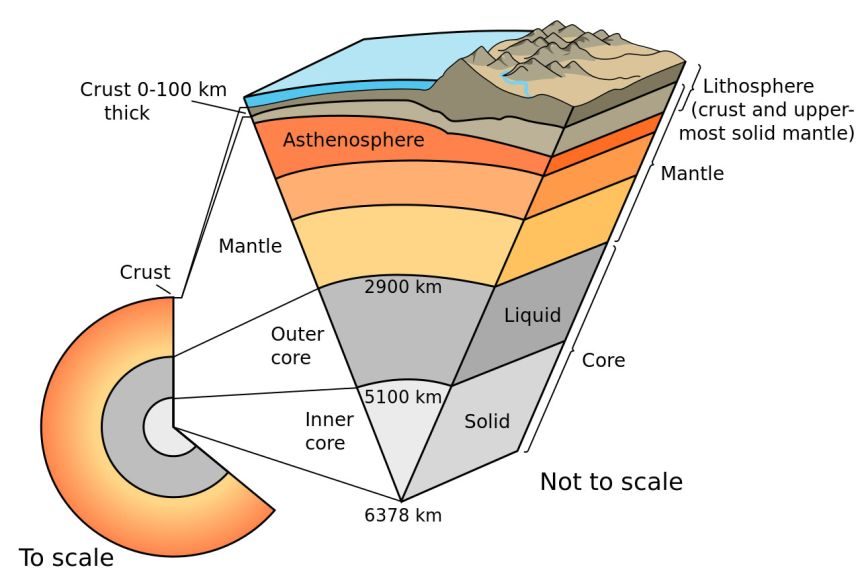
\includegraphics[width=9cm,height=7cm]{pics/cutaway-earth.jpg}
          \end{center} 
			 \qquad\tiny{(National Geographic)}
          }
         
\bigskip
\subhead{Goal.} Provide an \Oblue{accurate numerical approximation} of the time-dependent dynamics of a partially molten mantle.  

          \bigskip
          \subhead{Objective.} Provide a \Oblue{locally mass conservative} numerical framework for
          \begin{blist}
          \item The mechanics of a deformable solid matrix that is possibly partially molten.
          \item The transport phenomena of chemical species and energy in the presence of
porous media.
%\item Connecting the mechanics and the transport phenomena.
          \end{blist}
        %  \item Perform numerical simulation increase understanding of the physics.
          
\end{myslide}

% ============================================

\begin{myslide}
\heading{Mixture Theory for Mantle Dynamics}
\parbox{\textwidth}{\parbox{0.53\textwidth}{\raggedright
\subheading{Elementary Representative Volume.}
\centering
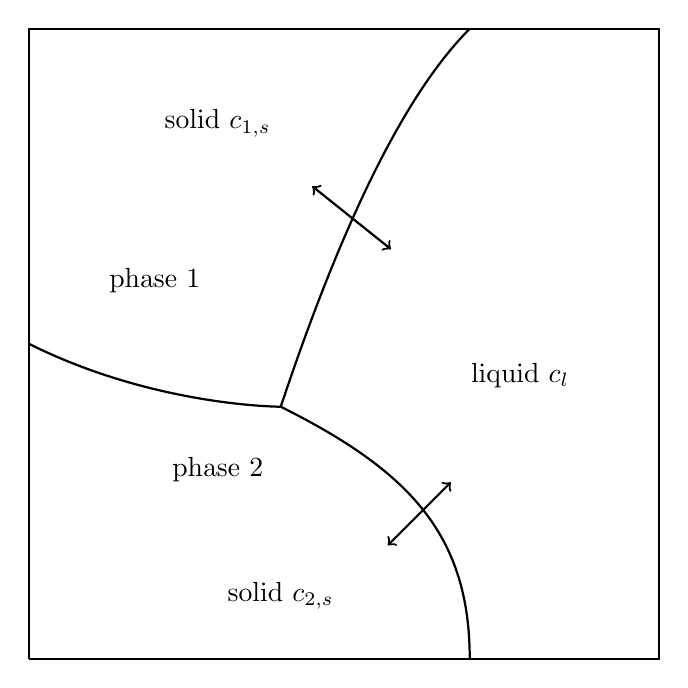
\begin{tikzpicture}[scale=0.4]
    \draw [thick] (0,0) -- (20,0) -- (20,20) -- (0,20) -- (0,0);
    \draw [thick] (0,10) .. controls (4,8) and (8,8) .. (8,8);
    \draw [thick] (8,8) .. controls (10,14) and (12,18) .. (14,20);
    \draw [thick] (8,8) .. controls (12,6) and (14,4) .. (14,0);
    
    %\draw (8,2) node {$\rho_2=c_{2,2}$};
    %\draw (6,17) node {$\rho_1=c_{1,1}=c_s$};
    \draw (8,2) node {solid $c_{2,s}$};
    \draw (6,17) node {solid $c_{1,s}$};
    %\draw (15,12) node {$c_{1,l}=c_{l}$};
    %\draw (15.6,6) node {$c_{2,l}$};

    \draw [thick, <->] (11.4,3.6) -- (13.4,5.6);
    \draw [thick, <->] (9,15) -- (11.5,13);
    %\draw [thick, <->] (15.6,7.6) -- (15.6,10.4);
    
    \draw (4,12) node {phase 1};
    \draw (6,6) node {phase 2};
    %\draw (16,16) node {liquid};
    \draw (15.6, 9) node {liquid $c_l$};
\end{tikzpicture}
}
\parbox{0.46\textwidth}{\raggedright
\subheading{Mixture Theory} %\Gray{(McKenzie 1984)}}
\vspace*{-0.3cm}
Both liquid ($l$) and solid ($s$) phases
exist at each point of the domain $\Omega$.

Define the \Maroon{mixture variable} (phase averaged) as:
\begin{equation*}
\begin{aligned}
\overline{\Psi} &= \phi \Psi_l + (1-\phi) \Psi_s \\ 
&= \Psi_s + \phi \Psi_r,\\
\Psi_r &= \Psi_l - \Psi_s. 
\end{aligned}
\end{equation*}}
}

\bigskip
\subhead{Extended Boussinesq Approximation.}
Density difference between phases are neglected expect
in the \Oorange{body force term}.

\subhead{Notation.}
\vspace{0.3cm}

\parbox{0.32\textwidth}{\raggedright
$c$ Mass concentration.\\
$\rho$ Density.\\
$h$ Specific enthalpy.\\
}\parbox{0.22\textwidth}{\raggedright
$p$ Pressure.\\
$\mu$ Viscosity.\\
$\mathbf{v}$ Velocity.
}\parbox{0.25\textwidth}{\raggedright
$T$ Temperature.\\
$\mathbf{g}$ Gravity.\\
$L$ Latent heat.
}\parbox{0.25\textwidth}{\raggedright
$c_p$ Specifc heat.\\
$\mathbf{g}$ Gravity.\\
$\alpha_\rho$ Thermal expansion.
}

\end{myslide}

\begin{myslide}
\heading{McKenzie Equations}

\subhead{A two-phase formulation of a viscous mantle.}

\begin{equation*}
\begin{alignedat}{3}
		  &\phi_l (\mathbf{v}_l - \mathbf{v}_s)
		  + \frac{k_{\phi_l}}{\mu_l}(\nabla p_l - \rho_f\mathbf{g})
	    &&= 0, \qquad &&\Maroon{\text{(Darcy's Law)}}\\
%		  &\nabla \cdot (\phi_l\mathbf{v}_l + \phi_s\mathbf{v}_s) &&=0,\\
		  &\nabla\bar p - \nabla \cdot \pmb{\tau}(\mathbf{v}_s) + \overline{\rho}\mathbf{g}&&= 0, \qquad &&\Maroon{\text{(Stokes Flow)}}\\
%		  &\mu_s\nabla \cdot \mathbf{v}_s - \phi_l(p_l - p_s) &&=0, 
&\frac{\partial \rho_l \phi}{\partial t} + \nabla\cdot (\rho_l \phi \mathbf{v}_l) &&= \Oorange{\Gamma} , \qquad && \\
&\frac{\partial \rho_s (1-\phi)}{\partial t} + \nabla\cdot (\rho_s (1-\phi) \mathbf{v}_s) &&= \Oorange{-\Gamma} , \qquad && 
\end{alignedat}
\end{equation*}
\Oblue{Deviatoric stress of mixture}
\begin{equation}\label{eq:deviatoricstress}
		  \pmb{\tau}(\mathbf{v}_s)
		  = 2\mu_s\phi_s\big( \tfrac{1}{2}(\nabla \mathbf{v}_s + \nabla \mathbf{v}_s^T) - \tfrac{1}{3}\nabla \cdot \mathbf{v}_s \mathbf{I}\big),
\end{equation}

\parbox{0.5\textwidth}{\raggedright
\subhead{Unknowns.} \\
\Oorange{Four} equations and \Oorange{six} unknowns.
\begin{blist}
\item Velocities $\mathbf{v}_l$ and $\mathbf{v}_s$.
\item Pressure $p_l$ and $p_s$.
\item Porosity $\phi$.
\item Melting source $\Gamma$.
\end{blist}
}\parbox{0.5\textwidth}{\raggedright
\subhead{Three parts.}
\begin{blist}
\item Static mechanic equations.
\item Transport of chemical species and energy.
\item Phase package or prescribed melting function.
\end{blist}
}

\end{myslide}

% ===================================================
\begin{myslide}
\heading{Degenerate Darcy-Stokes System}
\subhead{Pressure Potentials.}
\begin{equation*}
	q_l = p_l - \rho_l g z\quad\text{and}\quad q_s = p_s - \rho_l g z,
\end{equation*}
\begin{equation*}
		  p_l - p_s = q_l - q_s = \frac{1}{1-\phi}(q_l - q), \quad q=\bar{q}.
\end{equation*}
Then
\begin{alignat}{3}
		  &\phi\mathbf{v}_r + \frac{k_0\phi^{2+2\Theta}}{\mu_l}\nabla q_l &&= 0, \qquad \vspace*{0.5cm} && \Maroon{(\text{Darcy's Law})}\\
		  &\mu_s\nabla \cdot (\phi\mathbf{v}_r) + \frac{\phi}{1-\phi}(q_l-q) &&=0,
&&\Maroon{(\text{Conservation}}\\[-20pt]
& && &&\Maroon{\text{/Compaction})}\\[8pt]
  		  &\nabla q - \nabla \cdot \tau(\mathbf{v}_s) &&= -(1-\phi)\rho_r\mathbf{g},&&\Maroon{(\text{Stokes Flow})}\\
		  &\mu_s\nabla \cdot \mathbf{v}_s - \frac{\phi}{1-\phi}(q_l-q) &&=0, &&\Maroon{(\text{Compaction})}
\end{alignat}
\end{myslide}

\begin{myslide}
\heading{Scaled Variables}
\subhead{Problems.} When no melt, $\phi = 0$, 
\begin{nlist}
\item Darcy system degenerates when $\phi$ vanishes, lose bound on $q_l$.
\item Lose the conservation equation.
\item The condition number grows as $\phi \rightarrow 0$
\end{nlist}
         \subhead{Scaled Variables}\newline
          Define by Arbogast and Taicher [1]:
		  \begin{equation*}\label{eq:scaledVariables}
	\tilde{\mathbf{v}}_r = \phi_f^{-\Theta}\mathbf{v}_r
	\quad\text{and}\quad
	\tilde{q} = \phi^{1/2}q_l,
\end{equation*}
\subhead{The Space $H_{\phi}(\text{div})$}\newline
		  \Purple{$H_\phi(\Div;\Omega)$} is a \Cyan{Hilbert space} equipped with the \Maroon{weighted inner-product\vspace*{-6pt}}
\begin{equation*}
(\mathbf{u},\mathbf{v})_{H_\phi(\Div)} = (\mathbf{u},\mathbf{v}) + \big(\phi^{-1/2}\div(\phi^{1+\Theta}\mathbf{u}),\phi^{-1/2}\div(\phi^{1+\Theta}\mathbf{v})\big).
\end{equation*}\vspace*{-20pt}\newline
Moreover, $H(\Div;\Omega) = H_1(\Div;\Omega) \subset H_\phi(\Div;\Omega)$.
\end{myslide}

\begin{myslide}
\heading{Scaled Locally Mass Conservative Formulation}


\end{myslide}

\begin{myslide}
\heading{Transport of Chemical Species}

\end{myslide}

\begin{myslide}
\heading{Transport of Energy}

\end{myslide}

\end{document}
